\label{subseq:mm-library-choice}

\epigraph{\textit{Fair to say, there is no single algorithm or software that is the best for all types of linear systems}}{--- \citeauthor{list-of-sparse-direct-solvers}, \cite{list-of-sparse-direct-solvers}}

%Fair to say, there is no single algorithm or software that is the best for all types of linear systems \cite{list-of-sparse-direct-solvers}.\\


Nowadays, there exist many different and avaliable sparse direct solvers. Some of them are tunned for specific linear systems whereas others are targeted for the most general cases \cite{list-of-sparse-direct-solvers}. Some of them handle tree-task and node-data parallelism in different ways even within the same library depending on sizes of frontal matrices and other criteria \cite{wsmp}, \cite{mumps-manual}, \cite{superlu-manual}. Hence, parallel performance of a direct sparse method depends heavily on its specific implementation. Table \ref{table:mm-library-spec} represents a short summary of almost all available libraries capable to run on distributed-memory machines, at the time of writing, based on works \cite{list-of-sparse-direct-solvers} and \cite{petsc-web-page}.\\


\begin{table}[ht]
\small
\centering
\begin{tabular}{|c|c|c|c|c|}
\hline
Package & Method             & Matrix Types                 & \multicolumn{1}{c|}{\begin{tabular}[c]{@{}c@{}}PETSc\\ Interface\end{tabular}} & License      \\ \hline
Clique       & Multifrontal       & Symmetric      & \multicolumn{1}{c|}{\begin{tabular}[c]{@{}c@{}}Not \\ Officially\end{tabular}} & Open  \\ \hline
MF2          & Multifrontal       & \begin{tabular}[c]{@{}c@{}}Symmetric\\ pattern\end{tabular} & No              & -            \\ \hline
DSCPACK      & Multifrontal       & SPD                          & No              & Open \\ \hline
MUMPS        & Multifrontal       & General                      & Yes             & Open  \\ \hline
PaStiX       & Left looking & General                      & Yes             & Open  \\ \hline
PSPASES      & Multifrontal       & SPD                          & No              & Open \\ \hline
SPOOLES      & Left-looking       & \begin{tabular}[c]{@{}c@{}}Symmetric\\ pattern\end{tabular} & No              & Open \\ \hline
SuperLU\_DIST & Right-looking      & General                      & Yes             & Open  \\ \hline
symPACK      & Left-Right looking & SPD                          & No              & Open  \\ \hline
S+           & Right-lookin       & General                      & No              & -            \\ \hline

PARDISO         & Multifrontal       & General                      & No              & Commercial   \\ \hline

WSMP         & Multifrontal       & General                      & No              & Commercial   \\ \hline
\end{tabular}
\caption[A list of direct sparse linear solvers adapted for distributed-memory computations]{A list of direct sparse linear solvers adapted for distributed-memory computations, \cite{list-of-sparse-direct-solvers}, \cite{petsc-web-page}, where SPD - Symmetric Positive Definite}

\label{table:mm-library-spec}
\end{table}


It can be clearly observed, from Table \ref{table:mm-library-spec}, that only \acrshort{mumps}, PaStiX and SuperLU\_DIST cover requirements induced by \acrshort{grs}, see Chapter \ref{chapter:problem-statment}, in particular: open-source license and a direct interface to \acrshort{petsc}. Additionally, each development group of these solvers provides technical support for its software package. Therefore, it indirectly means that the solvers are maintainable. It is interesting to notice that all libraries, mentioned above, are implementations of different sparse direct methods, namely: multifrontal (\acrshort{mumps}), left-looking (PaStiX) and right-locking (SuperLU\_DIST). Moreover, PaStiX and SuperLU\_DIST use only static pivoting \cite{pastix-manual}, \cite{superlu-manual} whereas \acrshort{mumps} provides a full implementation of the threshold pivoting strategy \cite{mumps-manual}, described in Subsection \ref{subseq:pivot-hadling}.\\


To compare the libraries, a couple of flat-\acrshort{mpi} tests were performed using \acrshort{grs} matrix set and  \gls{hw1} compute-cluster. From now onwards, we refer to a flat-\acrshort{mpi} test as parallel factorizations of a matrix performed with varying values of the \acrshort{mpi} process count from 1 to 20 and conducted on a single compute-cluster node.\\


\acrshort{petsc} library was compiled and configured with \acrshort{mumps} (version 5.1.2), PasTiX (version 6.0.0) and SuperLU\_DIST (version 5.4) packages using their default parameter settings. An internal built-in \acrshort{petsc} profiler was used to measure execution time.  A time limit of 15 minutes was set up for each test-case to prevent blocking of a cluster compute-node from an unexpected long program execution. Results are summarized in Tables \ref{table:lc-cube-5-result}, \ref{table:lc-cube-64-result}, \ref{table:lc-k3-18-result} and in appendix \ref{app:app-lc} where numerical values are given in seconds.\\



\begin{table}[ht]
\centering
\begin{tabular}{|c|c|c|c|l|c|c|c|c|}
\cline{1-4} \cline{6-9}
MPI & MUMPS    & PaStiX   & SuperLU  &  & MPI & MUMPS    & PaStiX   & SuperLU  \\ \cline{1-4} \cline{6-9} 
1   & 7.02E-02 & 8.72E-02 & 3.17E+00 &  & 11  & 7.55E-02 & 8.89E-02 & 5.82E-01 \\ \cline{1-4} \cline{6-9} 
2   & 6.73E-02 & 7.10E-02 & 1.43E+00 &  & 12  & 7.61E-02 & 1.06E-01 & 4.37E-01 \\ \cline{1-4} \cline{6-9} 
3   & 6.36E-02 & 7.01E-02 & 1.07E+00 &  & 13  & 7.84E-02 & 9.72E-02 & 5.43E-01 \\ \cline{1-4} \cline{6-9} 
4   & 6.28E-02 & 7.11E-02 & 8.17E-01 &  & 14  & 8.06E-02 & 1.02E-01 & 4.22E-01 \\ \cline{1-4} \cline{6-9} 
5   & 6.50E-02 & 7.15E-02 & 7.51E-01 &  & 15  & 8.20E-02 & 1.19E-01 & 3.91E-01 \\ \cline{1-4} \cline{6-9} 
6   & 6.72E-02 & 7.62E-02 & 6.15E-01 &  & 16  & 8.07E-02 & 1.19E-01 & 4.44E-01 \\ \cline{1-4} \cline{6-9} 
7   & 6.91E-02 & 7.69E-02 & 6.48E-01 &  & 17  & 8.38E-02 & 1.22E-01 & 5.19E-01 \\ \cline{1-4} \cline{6-9} 
8   & 6.89E-02 & 8.17E-02 & 5.41E-01 &  & 18  & 8.40E-02 & 1.26E-01 & 3.77E-01 \\ \cline{1-4} \cline{6-9} 
9   & 7.50E-02 & 8.28E-02 & 5.02E-01 &  & 19  & 8.58E-02 & 1.33E-01 & 5.47E-01 \\ \cline{1-4} \cline{6-9} 
10  & 7.22E-02 & 8.52E-02 & 4.64E-01 &  & 20  & 8.64E-02 & 1.49E-01 & 3.39E-01 \\ \cline{1-4} \cline{6-9} 
\end{tabular}
\caption{Comparisons of parallel performance of  \textit{cube-5} matrix factorization using \acrshort{mumps}, PasTiX and SuperLU\_DIST solvers with their default parameter settings}
\label{table:lc-cube-5-result}
\end{table}


\begin{table}[ht]
\centering
\begin{tabular}{|c|c|c|c|l|c|c|c|c|}
\cline{1-4} \cline{6-9}
MPI & MUMPS    & PaStiX   & SuperLU  &  & MPI & MUMPS    & PaStiX   & SuperLU  \\ \cline{1-4} \cline{6-9} 
1   & 1.36E+00 & 1.39E+00 & time-out &  & 11  & 7.75E-01 & 8.15E-01 & time-out \\ \cline{1-4} \cline{6-9} 
2   & 1.00E+00 & 9.82E-01 & time-out &  & 12  & 7.81E-01 & 8.10E-01 & time-out \\ \cline{1-4} \cline{6-9} 
3   & 8.83E-01 & 1.06E+00 & time-out &  & 13  & 7.85E-01 & 8.35E-01 & time-out \\ \cline{1-4} \cline{6-9} 
4   & 8.17E-01 & 8.74E-01 & time-out &  & 14  & 7.85E-01 & 8.18E-01 & time-out \\ \cline{1-4} \cline{6-9} 
5   & 7.85E-01 & 8.50E-01 & time-out &  & 15  & 7.88E-01 & 8.46E-01 & time-out \\ \cline{1-4} \cline{6-9} 
6   & 8.06E-01 & 8.52E-01 & time-out &  & 16  & 7.81E-01 & 8.23E-01 & time-out \\ \cline{1-4} \cline{6-9} 
7   & 7.71E-01 & 8.33E-01 & time-out &  & 17  & 6.83E-01 & 8.49E-01 & time-out \\ \cline{1-4} \cline{6-9} 
8   & 7.66E-01 & 8.33E-01 & time-out &  & 18  & 7.96E-01 & 8.44E-01 & time-out \\ \cline{1-4} \cline{6-9} 
9   & 7.93E-01 & 8.35E-01 & time-out &  & 19  & 8.04E-01 & 8.65E-01 & time-out \\ \cline{1-4} \cline{6-9} 
10  & 8.07E-01 & 8.15E-01 & time-out &  & 20  & 6.85E-01 & 8.87E-01 & time-out \\ \cline{1-4} \cline{6-9} 
\end{tabular}
\caption{Comparisons of parallel performance of  \textit{cube-64} matrix factorization using \acrshort{mumps}, PasTiX and SuperLU\_DIST solvers with their default parameter settings}
\label{table:lc-cube-64-result}
\end{table}


\begin{table}[h!]
\centering
\begin{tabular}{|c|c|c|c|l|c|c|c|c|}
\cline{1-4} \cline{6-9}
MPI & MUMPS    & PaStiX   & SuperLU &  & MPI & MUMPS    & PaStiX   & SuperLU \\ \cline{1-4} \cline{6-9} 
1   & 1.55E+02 & 6.44E+01 & crashed &  & 11  & 1.77E+01 & 3.81E+01 & crashed \\ \cline{1-4} \cline{6-9} 
2   & 6.28E+01 & 4.84E+01 & crashed &  & 12  & 1.60E+01 & 3.75E+01 & crashed \\ \cline{1-4} \cline{6-9} 
3   & 5.06E+01 & 5.02E+01 & crashed &  & 13  & 1.42E+01 & 3.58E+01 & crashed \\ \cline{1-4} \cline{6-9} 
4   & 4.17E+01 & 4.50E+01 & crashed &  & 14  & 1.45E+01 & 3.59E+01 & crashed \\ \cline{1-4} \cline{6-9} 
5   & 2.52E+01 & 3.98E+01 & crashed &  & 15  & 1.47E+01 & 3.57E+01 & crashed \\ \cline{1-4} \cline{6-9} 
6   & 2.58E+01 & 4.29E+01 & crashed &  & 16  & 1.41E+01 & 3.52E+01 & crashed \\ \cline{1-4} \cline{6-9} 
7   & 2.65E+01 & 4.30E+01 & crashed &  & 17  & 1.54E+01 & 3.45E+01 & crashed \\ \cline{1-4} \cline{6-9} 
8   & 2.59E+01 & 3.73E+01 & crashed &  & 18  & 1.52E+01 & 3.31E+01 & crashed \\ \cline{1-4} \cline{6-9} 
9   & 1.95E+01 & 4.08E+01 & crashed &  & 19  & 1.52E+01 & 3.31E+01 & crashed \\ \cline{1-4} \cline{6-9} 
10  & 1.91E+01 & 3.81E+01 & crashed &  & 20  & 1.38E+01 & 3.16E+01 & crashed \\ \cline{1-4} \cline{6-9} 
\end{tabular}
\caption{Comparisons of parallel performance of \textit{k3-18} matrix factorization using \acrshort{mumps}, PasTiX and SuperLU\_DIST solvers with their default parameter settings}
\label{table:lc-k3-18-result}
\end{table}



Some problems were detected during  SuperLU\_DIST library testing. First of all, executions of \textit{cube-64} and \textit{k3-2} test-cases exceeded the set time limit. Secondly, it was noticed the library was crashing during processing of \textit{k3-18}, \textit{cube-645} and (partially) \textit{pwr-3d} test-cases. Debugging revealed that a segmentation fault occurred in function \textit{pdgstrf}  during the numerical factorization phase. Nonetheless, it is still unclear whether the problem was software or hardware specific. A solution or a reason of such program behavior has not been found at the moment of writing.\\


% FOR PRESENTATION: it can be due to wrong matrix representation in binary \acrshort{petsc} files. I ran into the same problem with METIS when it spinned the CPU for hours due to wrong CRS format

To complete comparison and evaluate parallel performance SuperLU\_DIST library, an additional test was conducted using a 2D formulation of the Poisson problem with \textit{100000} unknown. According to the results, SuperLU\_DIST managed to complete matrix factorizations within the set time limit without crashing, however, it showed abnormal jagged strong scaling behavior. Moreover, it turned out it was the slowest in comparison to the other solvers. The results are shown in Figure \ref{fig:5-point-stencil-solvers-comparison}.\\



\figpointer{\ref{fig:5-point-stencil-solvers-comparison}}
\begin{figure}[htpb]
  \centering
  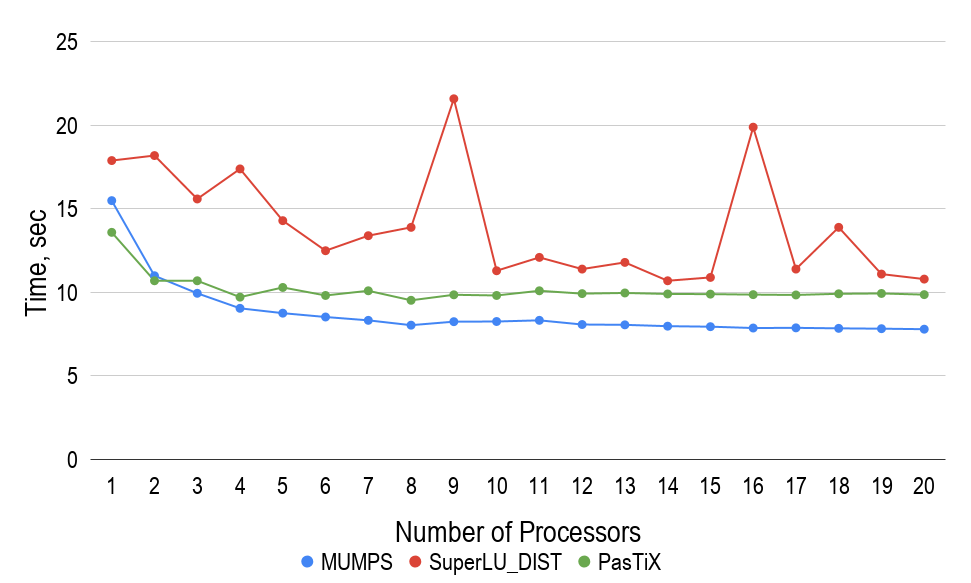
\includegraphics[width=0.85\textwidth]{figures/chapter-2/solvers-comparison-5-point-stencil.png}
\caption{Comparisons of parallel performance of \acrshort{mumps}, PasTiX and SuperLU\_DIST libraries during 5 point-stencil Poisson matrix (1000000  equations) factorizations
}
\label{fig:5-point-stencil-solvers-comparison}
\end{figure}

% FOR PRESENTATION: we think that 

According to the initial and additional tests, \acrshort{mumps} library showed the best parallel performance and scaling in contrast to the other solvers. No abnormal behavior during its operation was detected. In some cases, it only required to increase a multiplicative factor of estimated working space which was used to hold frontal matrices and factors $L$ and $U$ in memory. PaStiX was the second fastest solver according to the results of testing. However,  it was often considerably slower than \acrshort{mumps}. At the same time, SuperLU\_DIST showed the worst results. Additionally, as it was mentioned above, we experienced some technical problems during operation of this library.\\


A literature review showed quite contradictory results and conclusions. For example, \citeauthor{wsmp}, in \cite{wsmp}, came to nearly the same inference with respect to \acrshort{mumps}, as we did, comparing parallel performance of WSMP, \acrshort{mumps} and SuperLU\_DIST libraries using their matrix set. However, \citeauthor{mm-comparison-of-packages} showed, in \cite{mm-comparison-of-packages}, that SuperLU\_DIST spent the least amount of time on solving  systems of linear equations in contrast to the other solvers used in their work. It is needless to say that both research groups used different matrix sets and hardware. Nevertheless, it reveals a quite important fact that a selection of a particular method and its implementation can depend heavily on a specific matrix set.\\


In this section, we have compared different sparse direct methods and their concrete implementations using their default parameter settings with regard to \acrshort{grs} matrix set. Based on the obtained results and literature review, \acrshort{mumps} library is chosen for the rest of the study. In Section \ref{subseq:mumps-review}, we make an overview of the library and its specific traits. \\
